\documentclass[../Main.tex]{subfiles}
\begin{document}
\chapter{Blockchain}

\intro{

}

\section{Introduction}
\subsection{Motivation for Distributed Systems}
\begin{itemize}
    \item Scaling
    \item Location
    \item Fault-Tolerance
\end{itemize}
\subsection{Repository Structures}
\subsubsection{Monorepo}
\begin{itemize}
    \item Tight coupling
    \item Everyone sees code
    \item Encourages code sharing
    \item Scaling: large repos, specialized tooling
\end{itemize}
\subsubsection{Polyrepo}
\begin{itemize}
    \item Loose coupling
    \item Fine grained access control
    \item Encourages code sharing across organizations
    \item Scaling: many projects, special coordination
\end{itemize}
\subsection{Categorization}
\begin{itemize}
    \item Controlled DS
          \begin{itemize}
              \item 1 responsible org
              \item Low shurn
              \item Secure
              \item HA
              \item Homogenous or heterogeneous
              \item Mechanisms like:
                    Consistent hashing (DynamoDB, Cassandra), Master nodes, central coordinator,
                    Leader election (Zookeeper, Paxos, Raft), Replication (More replicas higher availability),
                    Transparancy principles apply
          \end{itemize}
    \item Fully Decentralized Systems
          \begin{itemize}
              \item N responsible orgs
              \item High churn
              \item Hostile env
              \item Unpredictable HA
              \item Heterogeneous
              \item Mechanisms like:
                    Consistent hashing (DHTSs), Flooding/broadcasting (Bitcoint),
                    Consistency (Weak DHTs, Nakamoto consensus Proof of Work), Proof of stage,
                    Replication principles apply, Transparency principles apply
          \end{itemize}
\end{itemize}

\section{Bitcoin}
\begin{itemize}
    \item Peer2Peer
    \item Smallest unit 0.00000001 BTC = 1 Satoshi
    \item Controlled Supply of BTC currently approx. 21 million
    \item Every transaction is broadcasted (660GB total)
    \item Proof of Work
    \item Weak anonymity
    \item Not controlled by single entity
\end{itemize}

\begin{figure}[H]
    \centering
    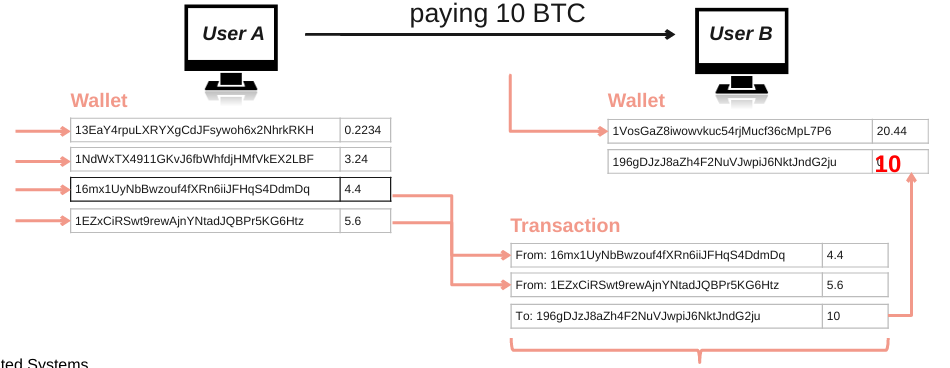
\includegraphics[width=0.75\linewidth]{Images/blockchain/bitcoin-transaction.png}
\end{figure}
\begin{figure}[H]
    \centering
    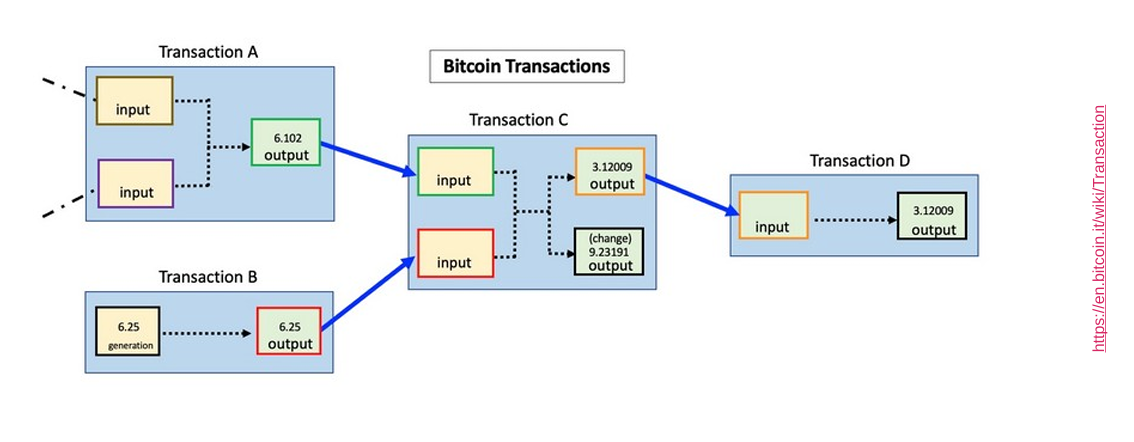
\includegraphics[width=0.75\linewidth]{Images/blockchain/bitcoin-transaction2.png}
\end{figure}

\section{Blockchain}
\begin{itemize}
    \item Transactions are chained within blocks
    \item Blocks approx. each 10 min
    \item Block has pointer to precious block
    \item Difficulty is adjustable
\end{itemize}
\begin{figure}[H]
    \centering
    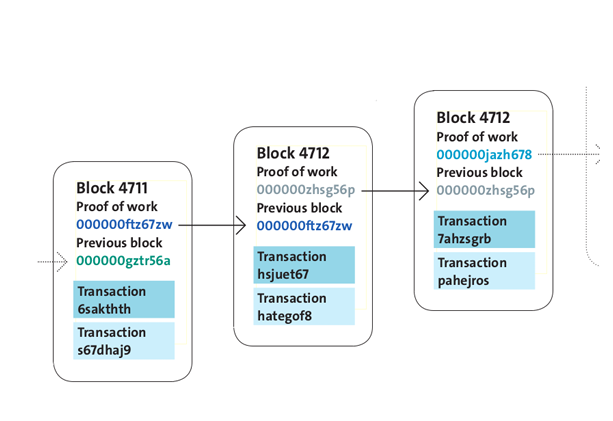
\includegraphics[width=0.75\linewidth]{Images/blockchain/blockchain.png}
\end{figure}
\begin{itemize}
    \item Disadvantages
          \begin{itemize}
              \item Power consumption
              \item Not Scalable (throughput comparison VISA)
              \item Anonymity (illegal activity)
              \item New features slow (Many hardforks)
              \item Scripting is limited
              \item 51\% attacks possible
          \end{itemize}
    \item Advantages
          \begin{itemize}
              \item Low transaction fees (about 1.2 satoshi per byte)
              \item Scalable as HW gets faster
              \item Anonymity (preservinc privacy)
          \end{itemize}
\end{itemize}

\begin{figure}[H]
    \centering
    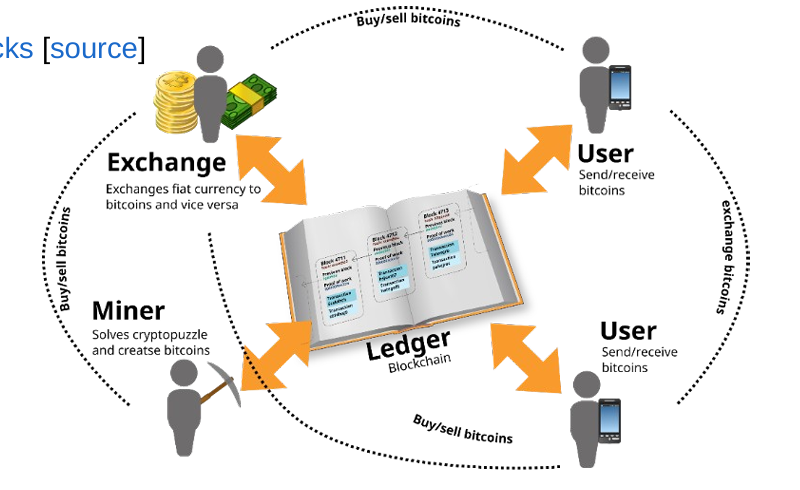
\includegraphics[width=0.75\linewidth]{Images/blockchain/bitcoin-stakeholders.png}
    \caption{Stakeholders}
\end{figure}

\subsection{Useful Links}
https://andersbrownworth.com/blockchain

\section{Account Abstration}
Ermöglich es Benutzerkonten programatisch zu steuern,
in dem Smart Contracs anstelle von privaten Schlüsseln die Logik für Tx übernehmen.

\begin{itemize}
    \item Motivation:
          \begin{itemize}
              \item EOA: User needs to manage keys and have eth for gas! This leads to poor UX
              \item Issues: Lost seed phrases, confusing gas payment, poor onboarding
              \item With AA: social login, account recovery, gas sponsorship, session keys, batched flows
          \end{itemize}
    \item Other chains with this feature: Solana, Sui
    \item Ethereum has moved its plans to implement native AA (Nov 2025 to TBA)
\end{itemize}

\begin{itemize}
    \item Core Features:
          \begin{itemize}
              \item Gasless Transactions (PayMaster)
              \item Fee Sponsorship (e.g other tokens like ERC-20)
              \item Social Recovery
              \item Key Management
              \item Session Keys (pre approved operations, auto approve tx, DeFi: automated trades within limits)
              \item Batched/Meta Tx (single click multistep workflows, atomic operations, ux, efficiency)
          \end{itemize}
\end{itemize}

\begin{itemize}
    \item Who builds infra?
          \begin{itemize}
              \item Wallet Teams (SA Implementations!)
                    \begin{itemize}
                        \item SimpleAccount, Argent, Soul Wallet, Biconomy, ZeroDev
                    \end{itemize}
              \item Bundlers (Permissionless Tx Aggr)
                    \begin{itemize}
                        \item Mainnet: Stackup, Alchemy, Pimlico, Etherspot
                        \item Testnet: Stackup, Alchemy dev
                        \item Anyone can run a bundler
                    \end{itemize}
              \item Paymasters (Gas Sponsorship Providers)
                    \begin{itemize}
                        \item DApps
                        \item Token projects (ERC-20)
                        \item Enterprise paymasters
                    \end{itemize}
              \item Tooling
                    \begin{itemize}
                        \item SDKs: Alchemy AA SDK, Biconomy SDK, ZeroDev SDK
                        \item Node Providers: Alchemy, Infura AA
                        \item Testing: Hardhat plugins, Foundry integration
                    \end{itemize}
          \end{itemize}
\end{itemize}

\begin{figure}[H]
    \centering
    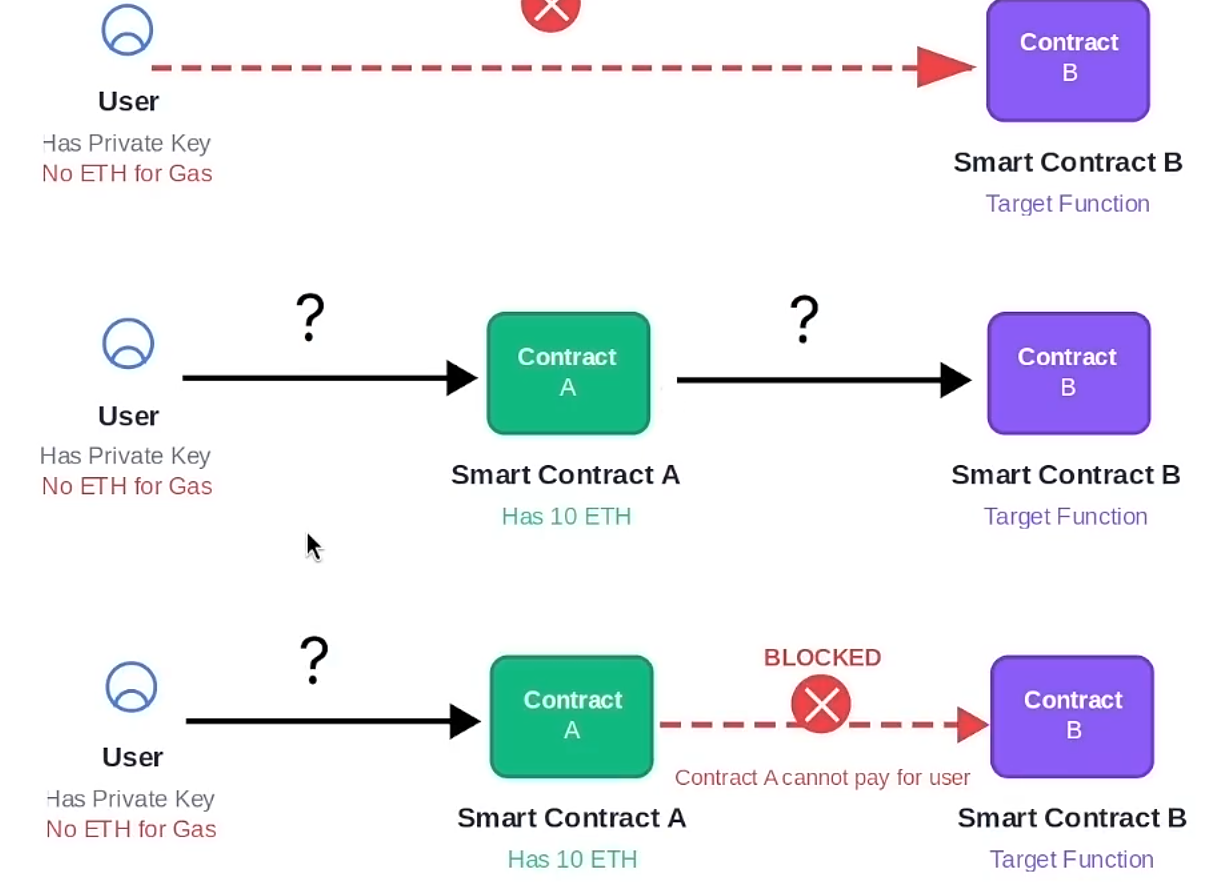
\includegraphics[width=0.75\linewidth]{Images/blockchain/account-abs-motivation.png}
    \caption{Currently, a default EOA cannot command a smart contract (contract a) to pay gas fees for e.g a contract b}
\end{figure}

\section{Ethereum}
\begin{itemize}
    \item Generalized Blockchain (Arithmetics etc)
    \item Protocols designed from scratch
    \item Founded in Zug
    \item Mining reward approx. block every 12x - 3\%
    \item Smart Contract = Turing Complete
    \item Smart Contracts have fees (Gas price)
\end{itemize}

\begin{figure}[H]
    \centering
    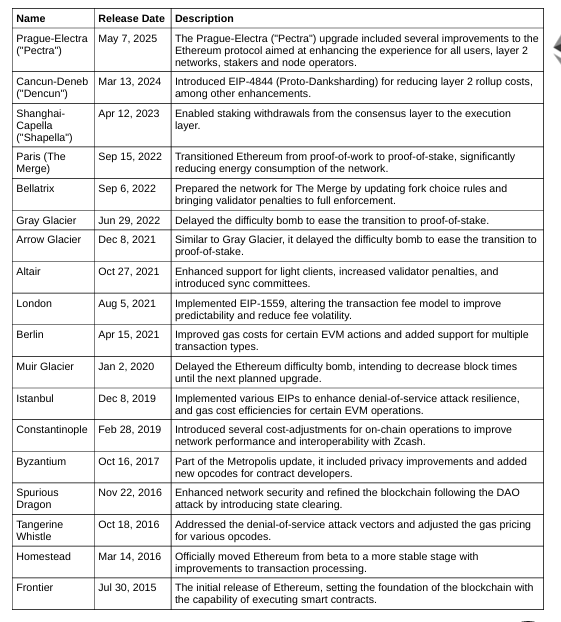
\includegraphics[width=0.75\linewidth]{Images/blockchain/eth-history.png}
    \caption{Ethereum History}
\end{figure}

\begin{itemize}
    \item ERC
    \begin{itemize}
        \item Stands for Ethereum Request for Comments
        \item Technical standard
        \item Community driven
    \end{itemize}
    \item EIP
    \begin{itemize}
        \item Ethereum Improvement Proposal
        \item Protocol changes/standards proposals
    \end{itemize}
\end{itemize}

\subsection{Stats (2024-25)}
\begin{itemize}
    \item 2nd in market cap - 480b USD
    \item Daily tx - 1500k per day (17tx/s avg)
    \item Node count - 10k
    \item Blocksize - 90-270KB
    \item 340m accounts
    \item Mining - 35m ETH staked, Top 12 (2023)
\end{itemize}

\subsection{Gas prices}
\begin{itemize}
    \item New: Algorithmically bases (approx. 36+2 gwei)
    \item Miner decides transaction at which price to include
    \item Tx market
    \item Gas price with low prio fee = longer waiting time until TX
    \item Every instruction within contract needs to be paid
    \item Gas price has to be fully paid: Otherwise state is reverted, ETH gone
    \item State modification more costly
\end{itemize}

\subsection{Smart Contract}
\begin{figure}[H]
    \centering
    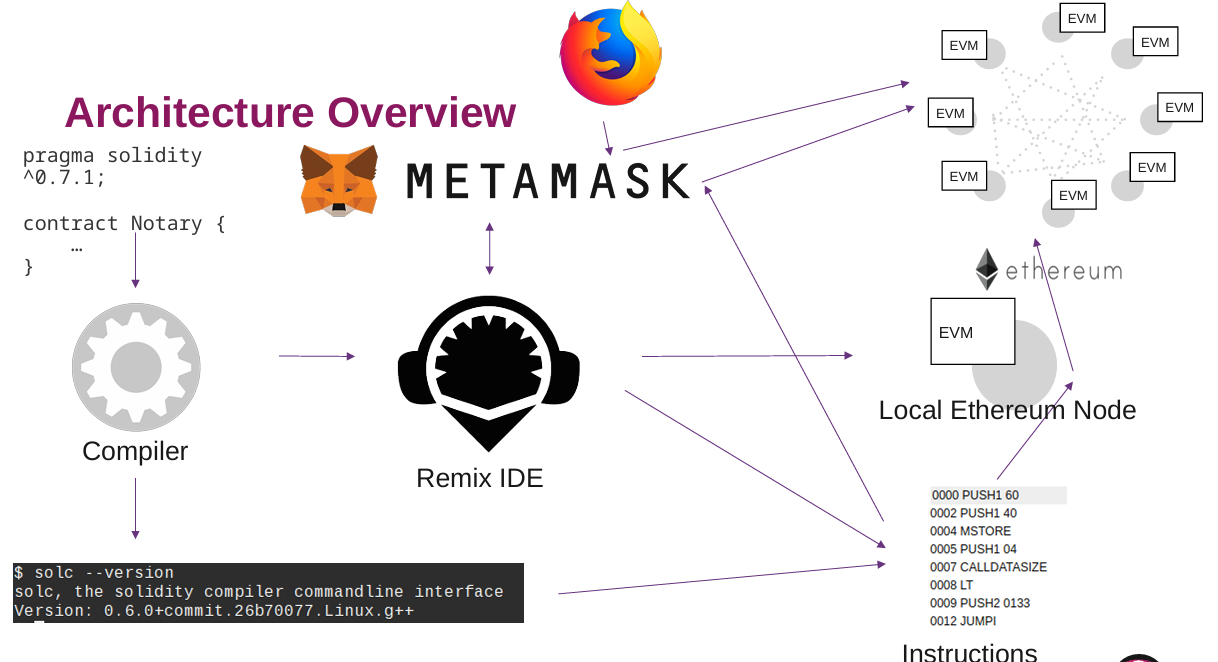
\includegraphics[width=0.75\linewidth]{Images/blockchain/smart-contract-arch.png}
    \caption{Smartcontract Dev Architecture}
\end{figure}

\begin{itemize}
    \item Computation on EVM (results are reproducable)
    \item Account-Based: 2 Types
          \begin{itemize}
              \item Both receive and send ether
              \item Externally controlled (standard accounts!)
                    \begin{itemize}
                        \item controlled by private keys
                        \item needs balance for gas!
                    \end{itemize}
              \item Contract accounts
                    \begin{itemize}
                        \item Never executed on their own
                        \item controlled by code
                        \item all action fired from externally controlled accounts
                    \end{itemize}
          \end{itemize}
\end{itemize}

\subsubsection{Account vs UTXO (Unspent Tx Output)}
\begin{itemize}
    \item Account-Based
          \begin{itemize}
              \item Global state stores list of accounts with balances and code
              \item Tx valid if sending account has balance
              \item If receiving account has code, code runs, state may be changed
          \end{itemize}
    \item UTXO
          \begin{itemize}
              \item Every input must be valid and not spent
              \item Total value of in >= total out
              \item Tx must have signature matching owner of input for every input
          \end{itemize}
\end{itemize}

\begin{figure}[H]
    \centering
    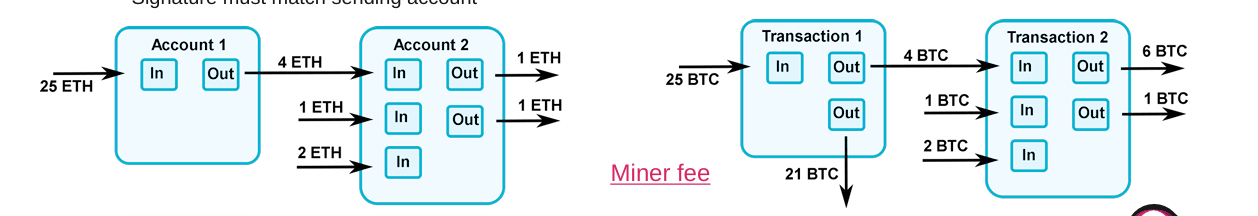
\includegraphics[width=0.75\linewidth]{Images/blockchain/account-utxo.png}
    \caption{Account-Based vs UTXO}
\end{figure}

\subsection{Off-Chain Account Abstraction (ERC-4337)}

\begin{itemize}
    \item In Production since March 2023
    \item 10-15\% gas cost increate vs EOA
    \item Infrastructure is not mature yet
    \item Centralization concerns: Concentration in bundlers and paymasters
    \item Security complexity: expand attack surface
    \item UX: 1.5x-11.7x slower transaction propagation
    \item Standards fragmentation: multiple wallet implementations 
    \item EIP-7702
    \begin{itemize}
        \item EOAs can set smart contract code by signing pointing to a delegation address
        \item Attach Smart Contract to EOA
        \item Fully compatible with 4337
    \end{itemize}
\end{itemize}

\begin{itemize}
    \item Core Concepts:
    \begin{itemize}
        \item Smart Contracts as Primary Accounts
        \item Programmable validation and authentication
        \item Seperation of signing and payment
    \end{itemize}
\end{itemize}

\begin{figure}[H]
    \centering
    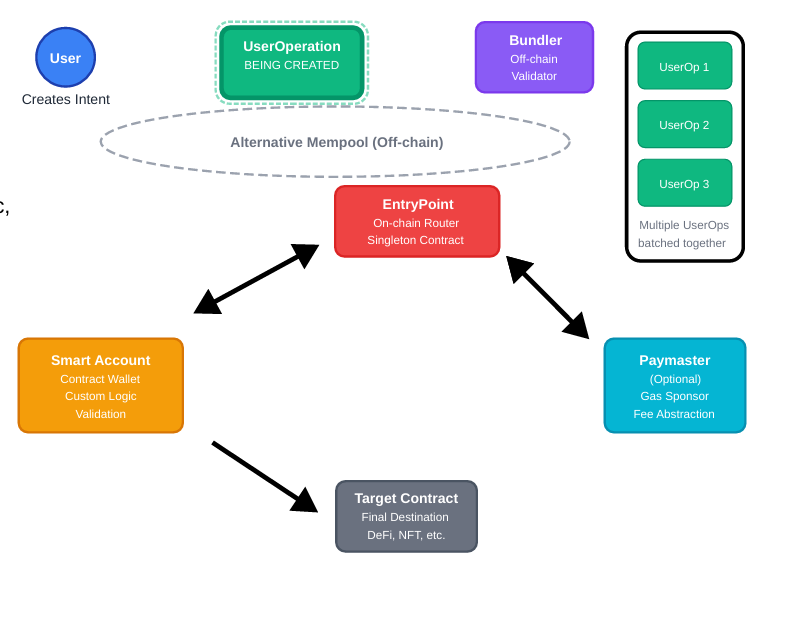
\includegraphics[width=0.75\linewidth]{Images/blockchain/erc-4337.png}
    \caption{Eth: Off Chain Account Abstraction}
\end{figure}
\begin{enumerate}
    \item User creates a UserOperation
          \begin{itemize}
              \item 14 additional AA fields
              \item Contains info for validation and exe
              \item Signed by user but not submitted to eth
              \item Put onto mempool
          \end{itemize}
    \item Bundler takes UserOperations
          \begin{itemize}
              \item Validation checks
              \item Creates optimized bundles to minimize gas
              \item Prepares bundle for EntryPoint
          \end{itemize}
    \item EntrPoint executes Bundle (OnChain!)
          \begin{itemize}
              \item Receives as regular eth tx
              \item Processes UserOps in 2 atomic phases
                    \begin{itemize}
                        \item Validation (ValidateUserOp) on smart account (state modifying)
                        \item Execution (execute()) with call data
                    \end{itemize}
              \item Manages gas accounting and refunds bundler immediately
              \item Any Userop fail = entire bunde reverts
          \end{itemize}
    \item Smart Account (validation and exe; On Chain!)
          \begin{itemize}
              \item Executed via ValidateUserOp by EntryPoint
              \item SA: Custom Validation logic
              \item If Paymaster present: EntryPoint validates gas sponsorship
              \item Validation may modify state (nonce, counters)
              \item If validation suceeds: EntryPoint calls execute()
              \item SA then forwards call to target contract
          \end{itemize}
\end{enumerate}

\subsubsection{Ether-Flow}
\begin{figure}[H]
    \centering
    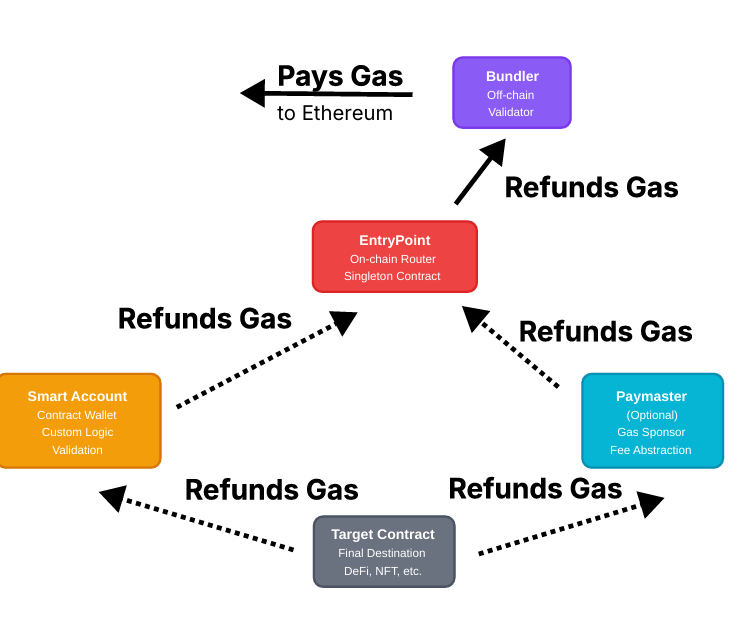
\includegraphics[width=0.75\linewidth]{Images/blockchain/ether-flow-4337.png}
    \caption{Shows how ether flows within 4337}
\end{figure}
\begin{itemize}
    \item Bundler payed by EntryPoint (only exe if bundler can be refunded)
    \item Typically the PayMaster pays
\end{itemize}

\subsection{Soldity}
Solidity is an object-oriented, high-level programming language used to write smart contracts,
most notably on the Ethereum blockchain and other compatible platforms.
It is designed to be compiled and executed by the Ethereum Virtual Machine (EVM),
enabling the creation of decentralized applications (dApps).

\begin{figure}[H]
    \centering
    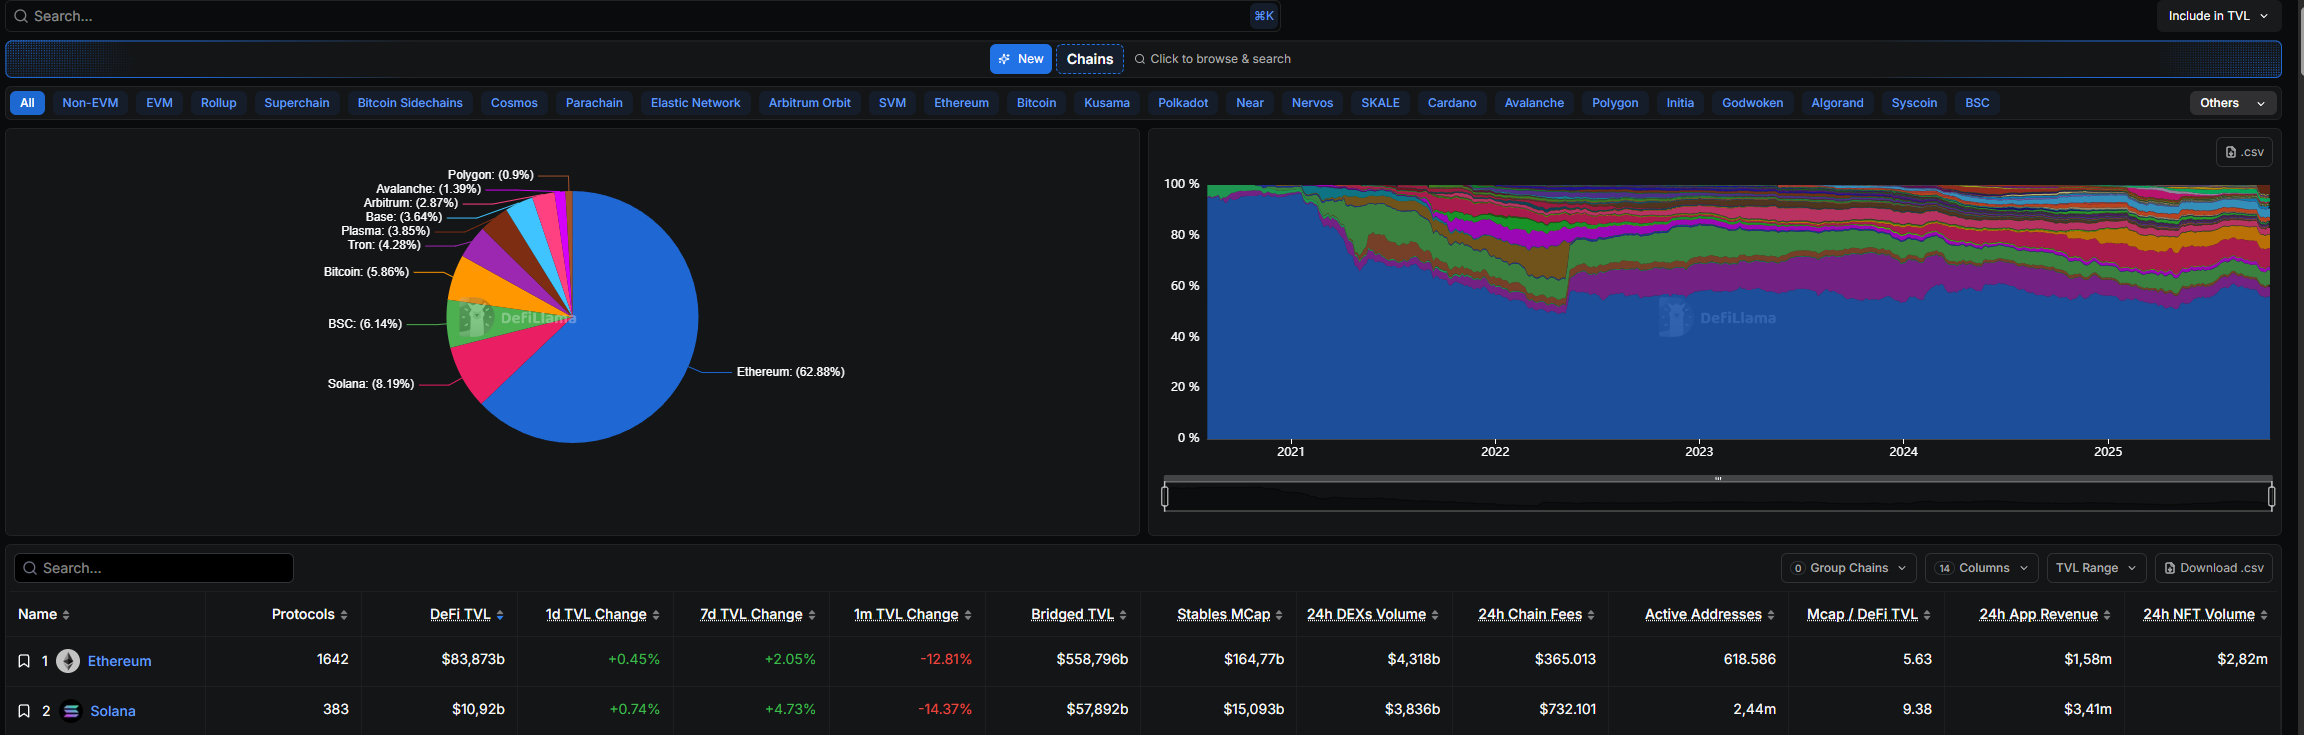
\includegraphics[width=0.75\linewidth]{Images/blockchain/defilama-smartcontract-chain.png}
    \caption{Currently, etherium is on place 1 (63\% total logged value), total value of all digital assets, indicator for trust. Bitcoin is low because of no smart contracts}
\end{figure}

\subsubsection{File Structure}
\begin{itemize}
    \item SPDX License Identifier (mandatory)
    \item Private code: UNLICENSED
    \item Version Pragma: pragma solidity \^ 0.8.30
    \item Battle-tested std-library: https://www.openzeppelin.com/solidity-contracts
    \begin{itemize}
        \item ERC20: Fungible Tokens
        \item ERC721: None Fungible Tokens (NFT)
        \item ERC1155: Both
    \end{itemize}
    \item Do not rewrite standards from scratch
\end{itemize}

\begin{itemize}
    \item State Variables are stored on blockchain (expensive to write)
    \item \begin{itemize}
        \item Storage: Persistend on blockchain, all state variables
        \item Memory: temporary, cleared after function, function parms, local vars
        \item calldata: read-only, cheapest for external func parms
        \item 
    \end{itemize}
    \item Function Visibility:
    \begin{itemize}
        \item Public: Globally callable
        \item Private: Only within contract
        \item Internal: Only within contract und abgeleitete contracts
        \item External: Only externally
    \end{itemize}
    \item Function Types:
    \begin{itemize}
        \item Pure: Only calcuations
        \item View: Read State
        \item Payable: Can receive or send ether
        \item (default): Can RW State
    \end{itemize}
    \item Important DT:
    \begin{itemize}
        \item address (20bytes, only payable addresses can exchange ether)
        \item No floats in solidity!
        \item Fixed sized arrays: bytes1-32
        \item Dynamic arrays: bytes
        \item Arrays: uint[] (dyn), uint[5] (fixed)
        \item string (UTF-8, expensive!)
        \item Hash Table: mapping(from => to), no iteration possible, cannot get list of keys
        \item Structs: struct name {field fieldname;}, composite types
        \item Enums: enum name {en1,en2,en3}, named constants
    \end{itemize}
    \item Constructor runs once when the contract is deployed
    \item Inhertitance:
    \begin{itemize}
        \item virtual: can be overriden
        \item override: overrides parent
        \item Always use OpenZeppeling base contracts
    \end{itemize}
\end{itemize}

\subsection{Useful Links}
\begin{itemize}
    \item Ethereum Whitepaper: https://ethereum.org/whitepaper/
    \item Metamask (Web3 browser plugin for eth tx in browsers, Js plugins injected: ether.js/Viem)
    \item Remix IDE
    \item Testnet: Sepolia https://sepolia.etherscan.io
    \item Faucet for Sepolia: https://sepolia-faucet.pk910.de
\end{itemize}

\subsubsection{Function Modifiers / Events}
\begin{itemize}
    \item Execute checks before functions
    \item Reusable access control
    \item Common in OpenZeppelin contracts
    \item \_\; placeholder = where function body executes
    \item Use modifier from OpenZeppelin
\end{itemize}
\begin{figure}[H]
    \centering
    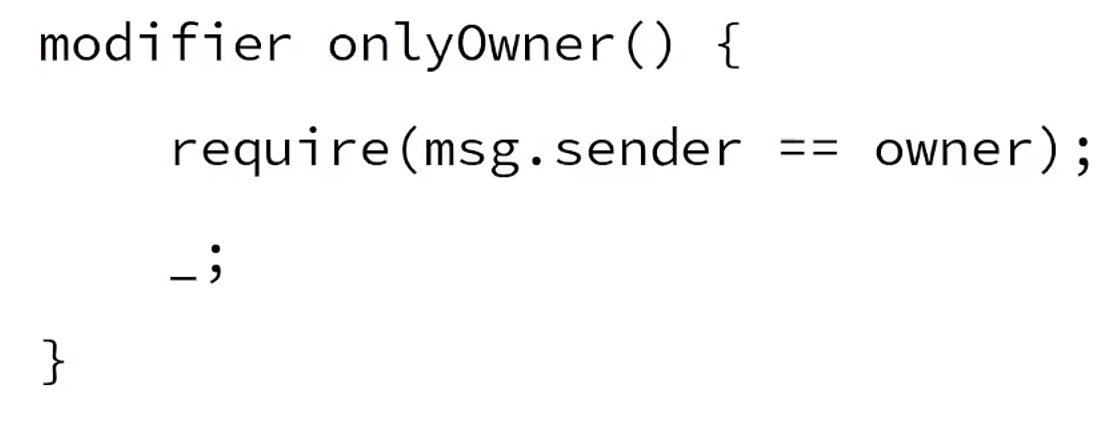
\includegraphics[width=0.75\linewidth]{Images/blockchain/sol-modifier-example.png}
    \caption{Custom Modifier Example}
\end{figure}
\begin{itemize}
    \item Events:
    \begin{itemize}
        \item One-Way communication to external world
        \item Used for logging or nofitication
        \item 
    \end{itemize}
\end{itemize}
\subsubsection{Error Handling}
\begin{itemize}
    \item Custom Errors (gas efficient)
    \begin{itemize}
        \item 
    \end{itemize}
    \item Require (expensive cause of strings, common, input validation)
    \item assert (for bug detection, uses all gas)
\end{itemize}

\subsubsection{Important Built-In Vars}
\begin{itemize}
    \item msg.sender
    \item msg.value
    \item block.timestamp
    \item block.number
    \item Units: wei, gewi, ether, seconds, minuts, hours, days
\end{itemize}

\end{document}
